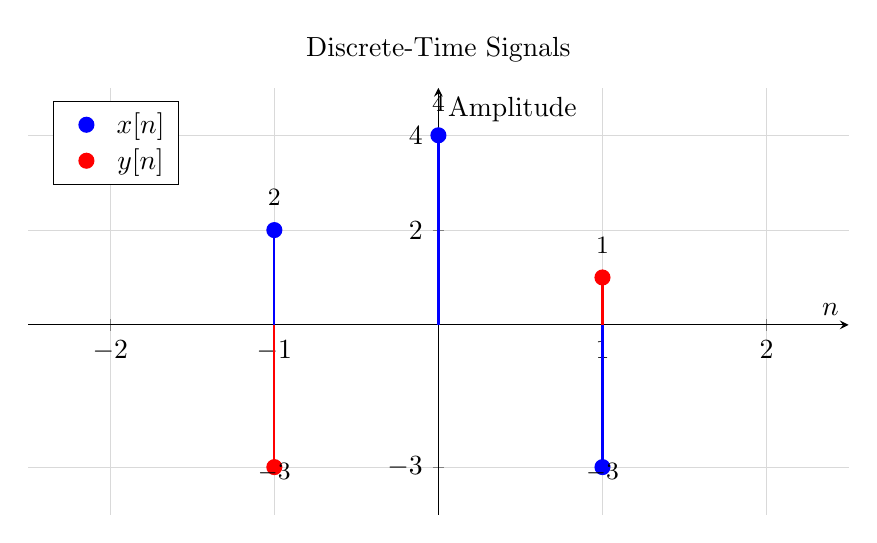
\begin{tikzpicture}
	\pgfplotsset{impulse/.style={ycomb,thick,mark=*,mark size=2.5pt}}
	\begin{axis}[
		width=12cm,
		height=7cm,
		title={Discrete-Time Signals},
		xlabel={$n$},
		ylabel={Amplitude},
		axis lines=middle,
		xmin=-2.5, xmax=2.5,
		ymin=-4, ymax=5,
		xtick={-2,-1,0,1,2},
		ytick={-3, 2, 4},
		grid=major,
		grid style={line width=.1pt, draw=gray!30},
		legend pos=north west,
		]
		\addplot[impulse, blue, nodes near coords,
		every node near coord/.style={yshift=5pt,font=\small,text=black}] 
		coordinates {(-1,2) (0,4) (1,-3)};
		\addlegendentry{$x[n]$};
		
		\addplot[impulse, red, nodes near coords,
		every node near coord/.style={yshift=5pt,font=\small,text=black}] 
		coordinates {(-1,-3) (1,1)};
		\addlegendentry{$y[n]$};
	\end{axis}
\end{tikzpicture}